% !TEX options=--shell-escape
	\documentclass{article}
	\usepackage{amsmath,amssymb}
	\usepackage[inline]{enumitem}
	\usepackage{blindtext}
	\usepackage{booktabs}
	\usepackage{graphicx}
	\usepackage{xcolor}
	\usepackage[vmargin = 1.5in, top = 1in, bottom = 1.2in, letterpaper]{geometry}
	\usepackage{listings}
	\usepackage{courier}
	\usepackage{multicol}
	\usepackage{multirow}
	\usepackage{bm}
	\usepackage[labelformat=simple]{subcaption}
	\renewcommand\thesubfigure{(\alph{subfigure})}
	\usepackage{minted}
	\usepackage{fvextra}
	\definecolor{bg}{rgb}{0.95,0.95,0.95}
	\newminted{r}{mathescape, breaklines, linenos = true, bgcolor = bg, fontsize = \footnotesize}
	\usemintedstyle{tango}
	% \lstset{
	% basicstyle = \small\tt,
	% keywordstyle = \tt\color{blue},
	% commentstyle = \it\color[cmyk]{1,0,1,0},
	% stringstyle = \tt\color[RGB]{128,0,0},
	% %frame = single,
	% backgroundcolor = \color[RGB]{245,245,244},
	% breaklines,
	% extendedchars = false,
	% xleftmargin = 2em,
	% xrightmargin = 2em,
	% aboveskip = 1em,
	% tabsize = 4,
	% showspaces = false
	% }
	\newcommand\inner[2]{\left\langle{#1},{#2}\right\rangle}
	\DeclareMathOperator{\Corr}{Corr}
	\DeclareMathOperator{\Cov}{Cov}
	\DeclareMathOperator{\Var}{Var}
	\DeclareMathOperator{\E}{E}



	\begin{document}
	
	% \newfontfamily\courier{Courier New}

	
	\title{STAT 501 Homework 8}
	\author{Multinomial}
	\maketitle

	First we standardized the data and use the standardized data in the clustering.
	\begin{rcode}
women <- read.table("women-track-records.dat",
                    header=F, col.names=c("x1", "x2", "x3", "x4", "x5","x6","x7", "Country"))

men <- read.table("men-track-records.dat",
                    header=F, col.names=c("x1", "x2", "x3", "x4", "x5","x6","x7", "x8", "Country"))

women.country <- women$Country
men.country <- men$Country

women <- women[,-ncol(women)]
men <- men[,-ncol(men)]

# standardize the data
women <- scale(women)
men <- scale(men)
	\end{rcode}
	
	\begin{itemize}[leftmargin = 0 em]
	
	\item Hierarchical Clustering

	Before doing hierarchical clustering, we mapped the data to the sphere. In this way the Euclidian distance is just the correlation similarity distance for the standardized the data. We adopted complete linkage in hierarchical clustering for men and women. The hierarchical tree is shown in Figure~\ref{tree} and we display the clustering result with 3 clusters in Figure~\ref{hc} using the 2 LDs by LDA.
	\begin{rcode}
#  Sphere the data for correlation similarity distance
men.sphere<-t(apply(men,1,FUN= function(x) (x - mean(x))/sqrt(sum((x - mean(x))^2))))
women.sphere<-t(apply(women,1,FUN= function(x) (x - mean(x))/sqrt(sum((x - mean(x))^2))))

#  Use complete linkage, this is also the default method
hc.men <- hclust(dist(men.sphere),method="complete")
plot(hc.men, label = men.country,
main = "Complete Linkage Cluster Analysis: Men Track Records Data") 

hc.women <- hclust(dist(women.sphere),method="complete")
plot(hc.women, label = women.country,
     main = "Complete Linkage Cluster Analysis: Women Track Records Data") 

#  Use canonical discriminants to display the clusters.
#  The first function computes linear canonical discriminants and
#  the second function is used to plot the computed scores.
library(MASS)
#  Compute canonical discriminant scores and display 2-dimensional
#  projections of the clusters

hc.men.lda <- lda(men, cutree(hc.men, 3))  
plot(hc.men.lda)

hc.women.lda <- lda(women, cutree(hc.women, 3))  
plot(hc.women.lda)
	\end{rcode}

\begin{figure}[!htb]
          \begin{subfigure}[b]{\linewidth}
            \centering
            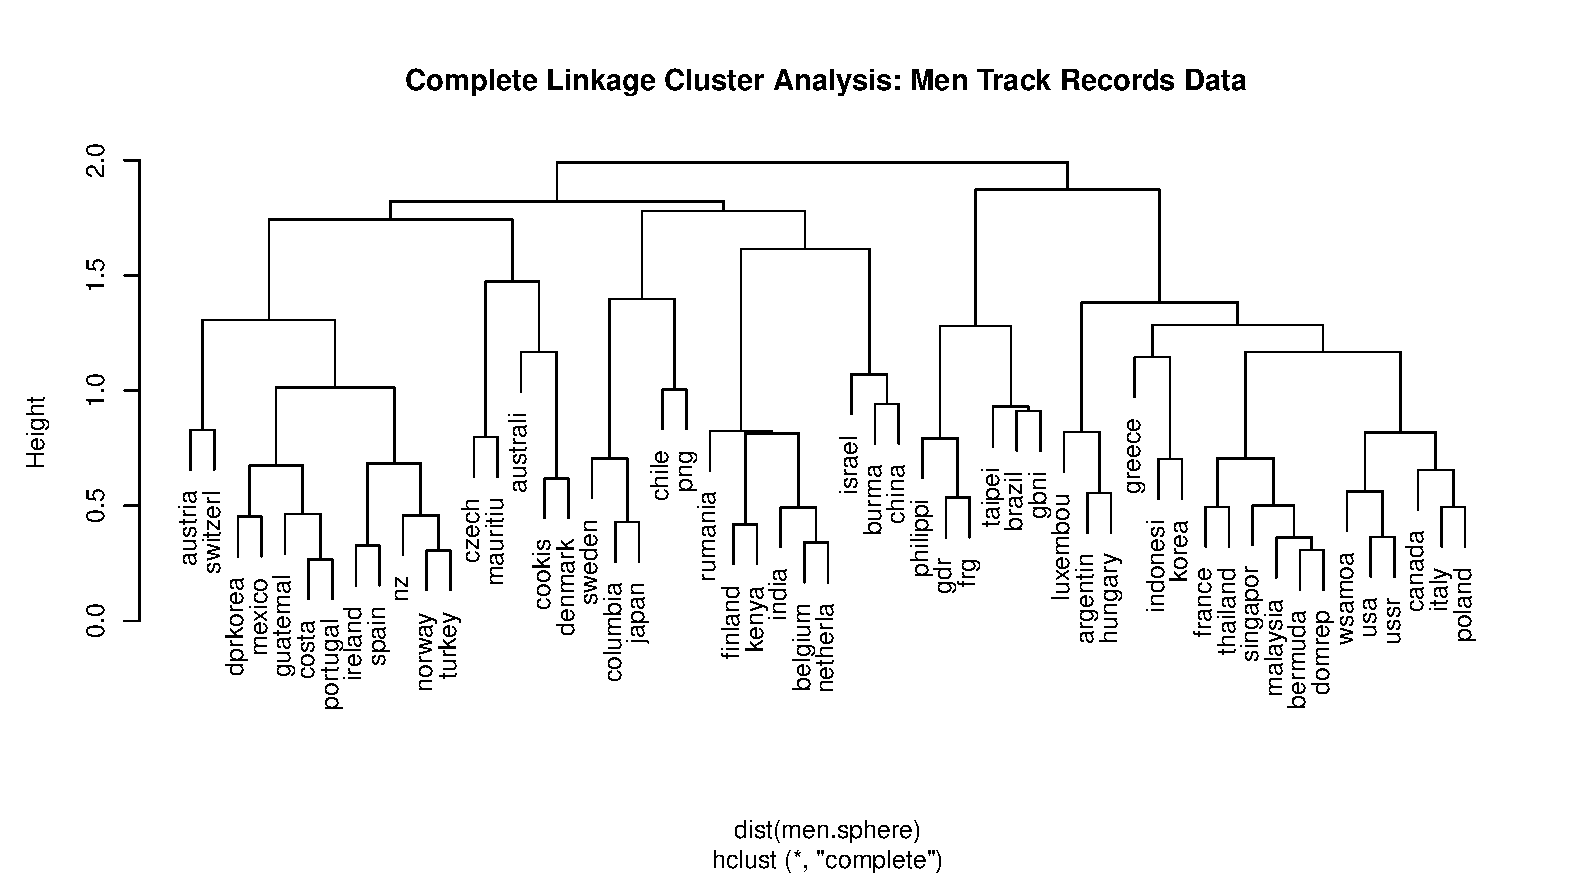
\includegraphics[width = 0.9\textwidth]{men_tree.eps}
            \caption{}
          \end{subfigure}%
          \\
          \begin{subfigure}[b]{\linewidth}
            \centering
            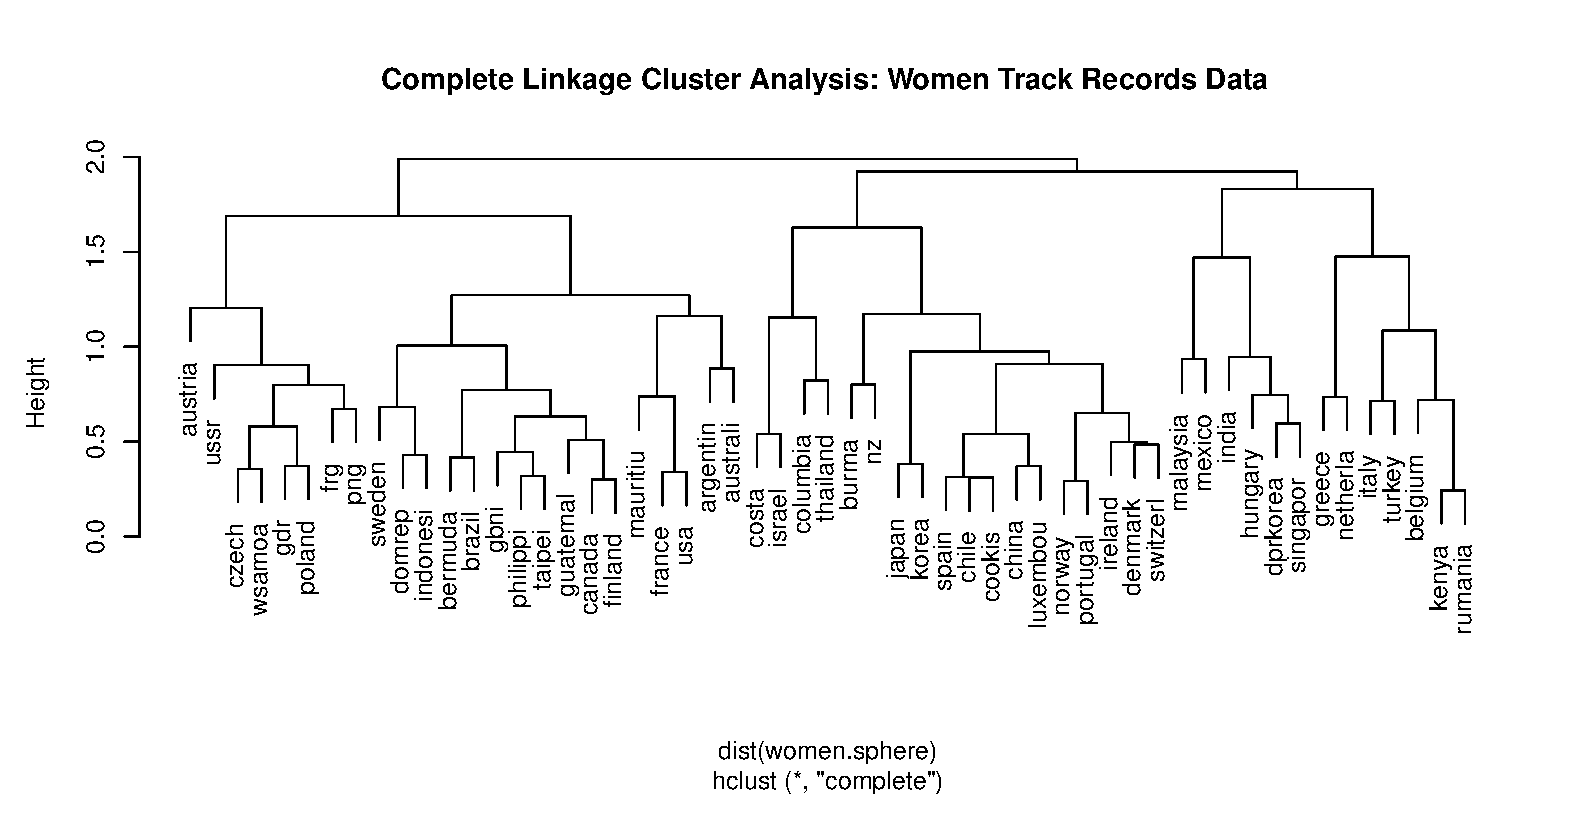
\includegraphics[width = 0.9\textwidth]{women_tree.eps}
            \caption{}\
          \end{subfigure}
          \caption{Hierarchical clustering tree}
          \label{tree}
\end{figure}

\begin{figure}[!htb]
          \begin{subfigure}[b]{0.5\linewidth}
            \centering
            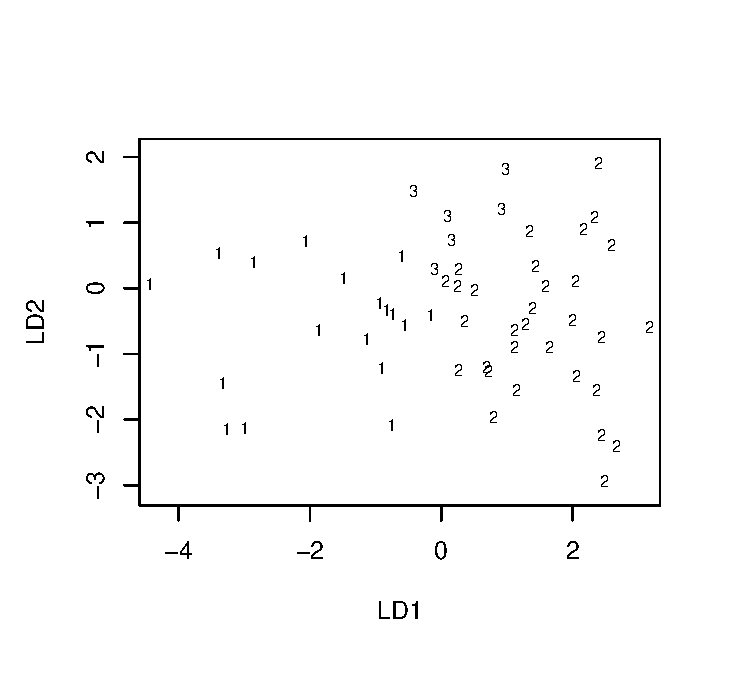
\includegraphics[width = \textwidth]{men_hc.eps}
            \caption{men}
          \end{subfigure}%
          \begin{subfigure}[b]{0.5\linewidth}
            \centering
            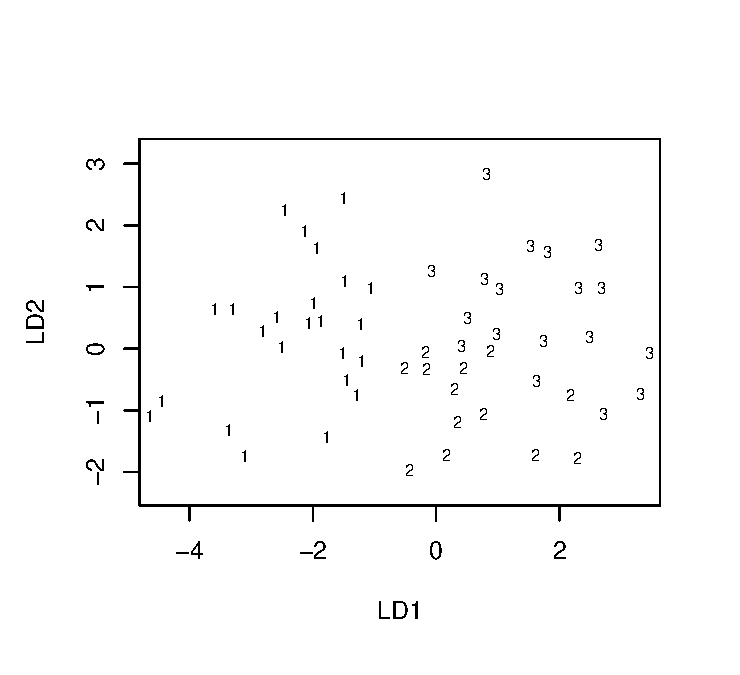
\includegraphics[width = \textwidth]{women_hc.eps}
            \caption{women}
          \end{subfigure}
          \caption{Hierarchical clustering results}
          \label{hc}
\end{figure}


\newpage
\item k-means

We use the results of hierarchical clustering with ward linkage as our initial for k-means. Then we display the results from k-means with 3 clusters using the 2 LDs from LDA in Figure~\ref{km}.
\begin{rcode}
#  Compute K-means cluster analysis starting with results from hclust
kmnsinithcl <- function(x.data, nclus, ncut = nclus, hcl.tree)
{
  x.hcl <- hcl.tree
  x.cl <- cutree(x.hcl, k = ncut)
  data.x <- data.frame(x.data, cl = x.cl)
  means <- aggregate(. ~ cl, data = data.x, FUN = mean)
  return(kmeans(x.data,centers= means[, -1]))
}

hc.men2 <- hclust(dist(men.sphere),method="ward.D2")
km.men <- kmnsinithcl(men, nclus = 3, ncut = 3, hcl.tree = hc.men2)
km.men.lda <- lda(men, km.men$cluster)
plot(km.men.lda)

hc.women2 <- hclust(dist(women.sphere),method="ward.D2")
km.women <- kmnsinithcl(women, nclus = 3, ncut = 3, hcl.tree = hc.women2)
km.women.lda <- lda(women, km.women$cluster)
plot(km.women.lda)
\end{rcode}

\begin{figure}[!htb]
          \begin{subfigure}[b]{0.5\linewidth}
            \centering
            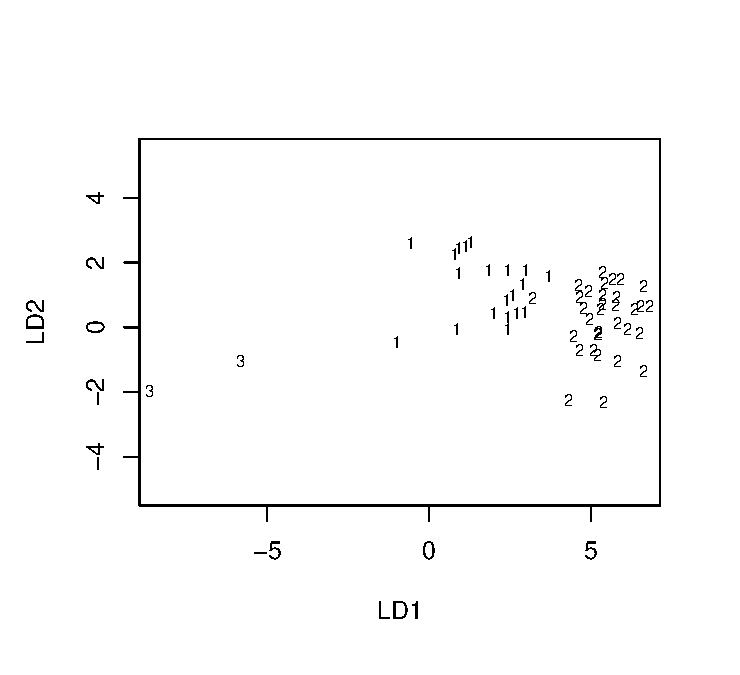
\includegraphics[width = \textwidth]{men_km.eps}
            \caption{men}
          \end{subfigure}%
          \begin{subfigure}[b]{0.5\linewidth}
            \centering
            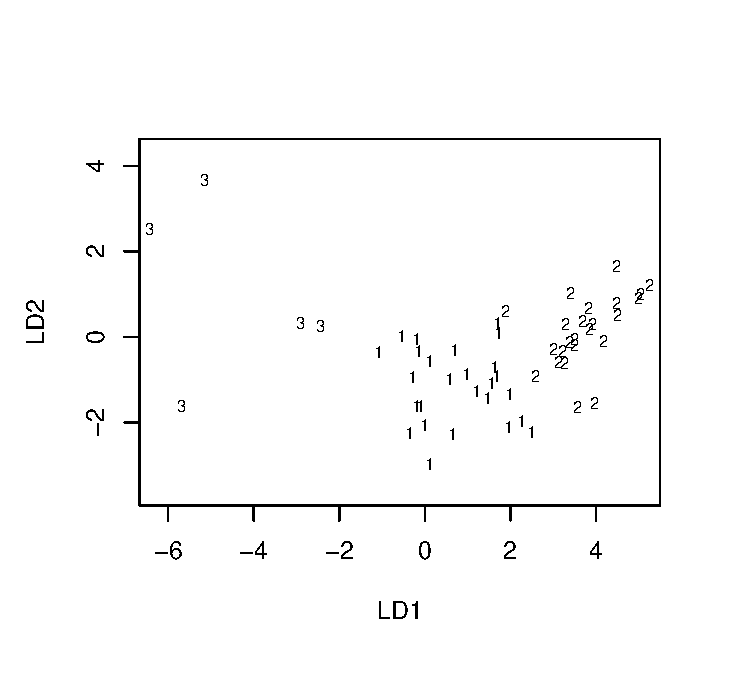
\includegraphics[width = \textwidth]{women_km.eps}
            \caption{women}
          \end{subfigure}
          \caption{k-means clustering results}
          \label{km}
\end{figure}

\item Model based clustering

For model based clustering, we use BIC to pick the model and number of clusters. In Figure~\ref{bic} we can see, for men, model VEE and 2 clusters is the best, while model VEV and 2 clusters for women is the best. The display of clustering is shown in Figure~\ref{mcl}.

\begin{rcode}
#  Model based clustering based on the assumption that 
#  the data were sampled from a mixture of multivariate normal
#  distributions with common covariance matrix 

library(mclust)

mcl.men <- Mclust(men)
plot(mcl.men$BIC)
plot.Mclust(mcl.men, what = "classification")

mcl.women <- Mclust(women)
plot(mcl.women$BIC)
plot.Mclust(mcl.women, what = "classification")
\end{rcode}

\begin{figure}[!htb]
          \begin{subfigure}[b]{0.5\linewidth}
            \centering
            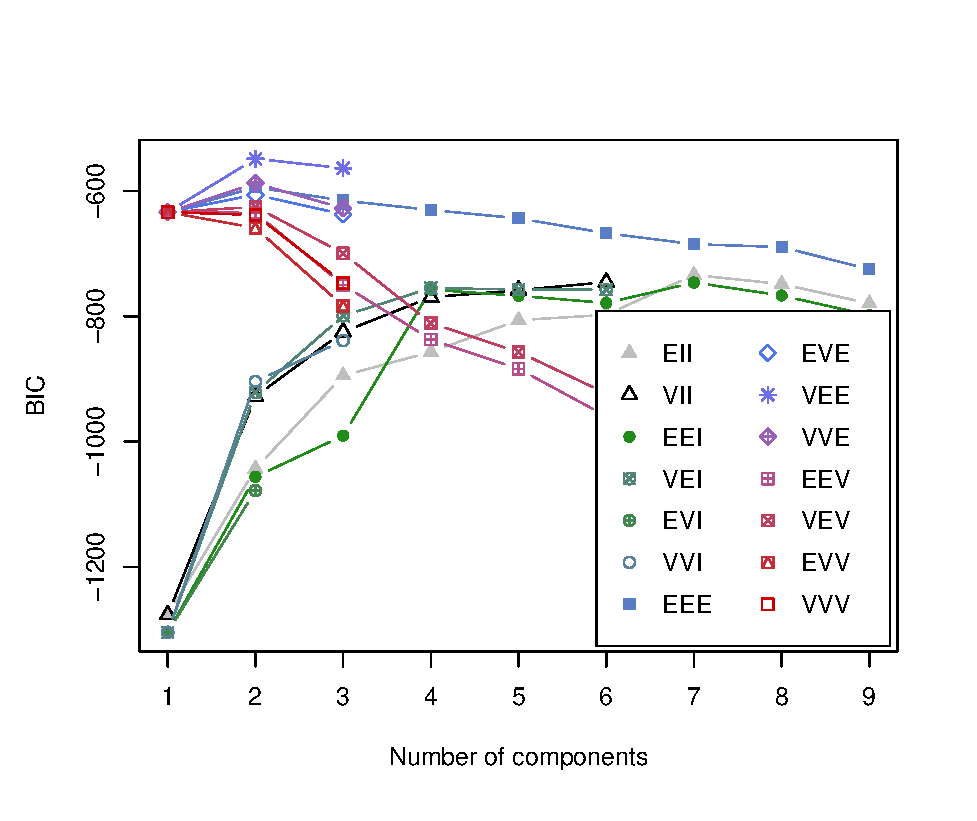
\includegraphics[width = \textwidth]{bic.eps}
            \caption{men}
          \end{subfigure}%
          \begin{subfigure}[b]{0.5\linewidth}
            \centering
            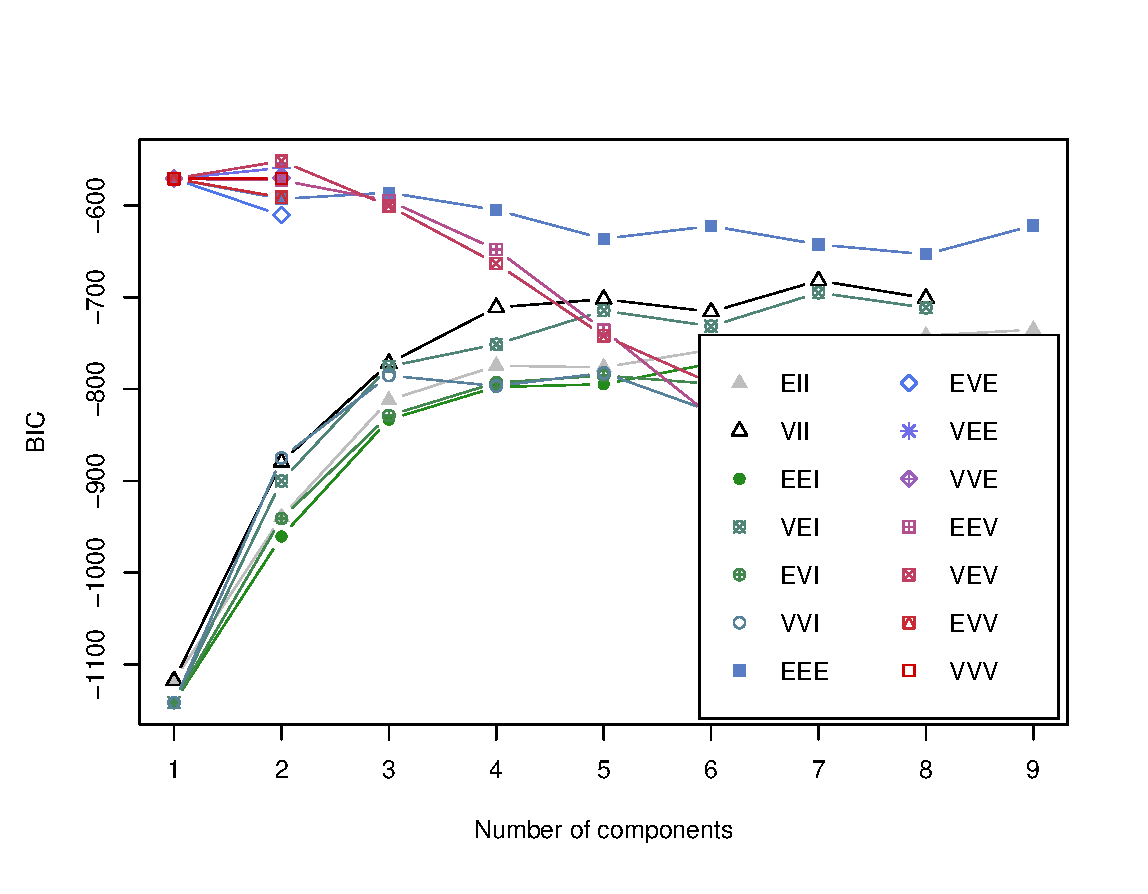
\includegraphics[width = \textwidth]{bic_women.eps}
            \caption{women}
          \end{subfigure}
          \caption{BIC for model selection}
          \label{bic}
\end{figure}

\begin{figure}[!htb]
          \begin{subfigure}[b]{\linewidth}
            \centering
            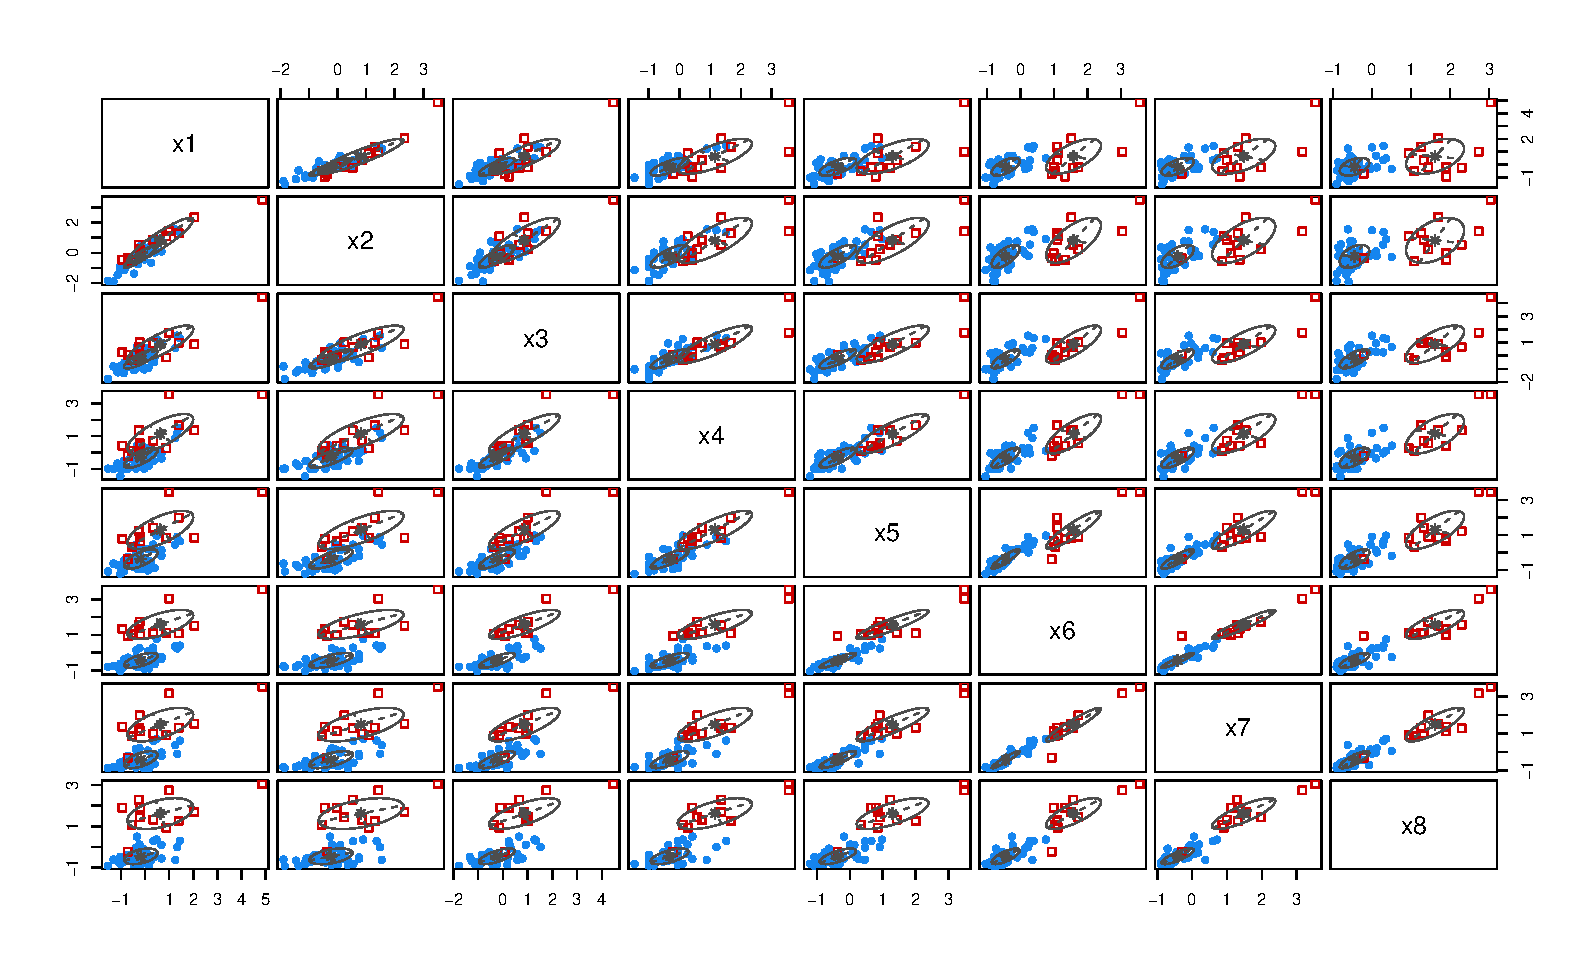
\includegraphics[width = 0.9\textwidth]{men_clust.eps}
            \caption{men}
          \end{subfigure}%

          \begin{subfigure}[b]{\linewidth}
            \centering
            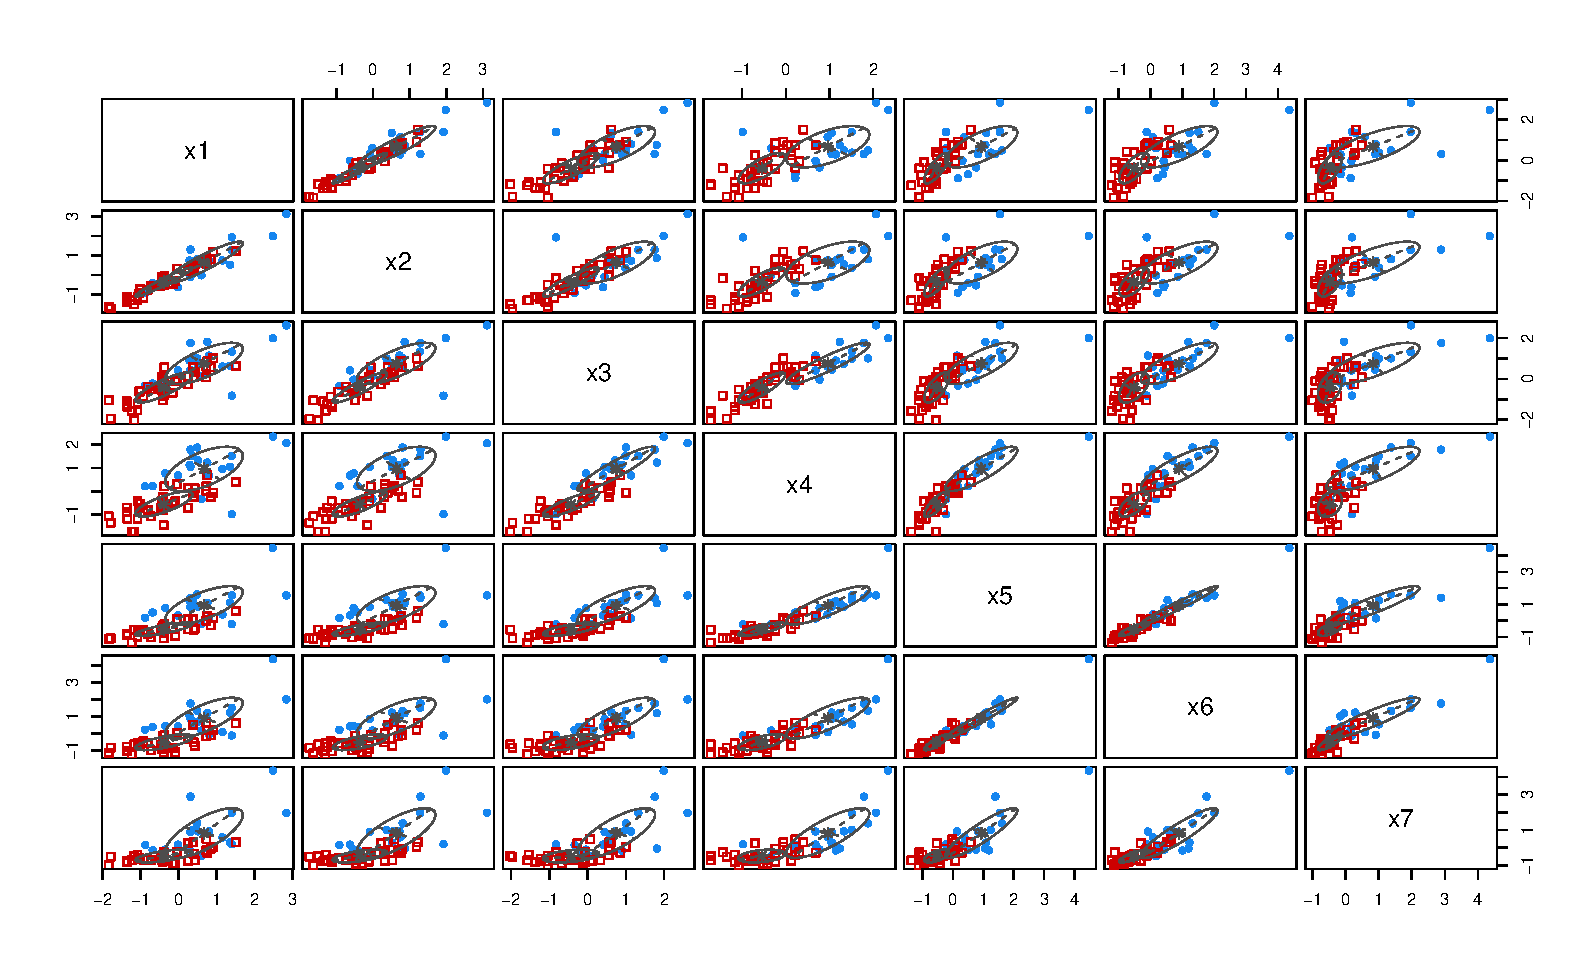
\includegraphics[width = 0.9\textwidth]{women_mclust.eps}
            \caption{women}
          \end{subfigure}
          \caption{Model based clustering results}
          \label{mcl}
\end{figure}




	
 \end{itemize}

 \newpage

 \noindent Comment: 

 The clustering results using 3 methods shows some differences in the clusters patterns between men and women. However we can see from the results using 3 methods that there might be 2 clusters for both women and men. 









	
	
	
	\end{document}